
\documentclass[a4paper, 10pt, twoside]{article}

\usepackage[top=1in, bottom=1in, left=1in, right=1in]{geometry}
\usepackage[utf8]{inputenc}
\usepackage[spanish, es-ucroman, es-noquoting]{babel}
\usepackage{setspace}
\usepackage{fancyhdr}
\usepackage{lastpage}
\usepackage{amsmath}
\usepackage{amsfonts}
\usepackage{amsthm}
\usepackage{verbatim}
\usepackage{fancyvrb}
\usepackage{graphicx}
\usepackage{float}
\usepackage{enumitem} % Provee macro \setlist
\usepackage{tabularx}
\usepackage{multirow}
\usepackage{hyperref}
\usepackage{xspace}
\usepackage{ulem} % Provee macro \uwave
\usepackage[toc, page]{appendix}


%%%%%%%%%% Constantes - Inicio %%%%%%%%%%
\newcommand{\titulo}{Trabajo Práctico 1}
\newcommand{\materia}{Bases de Datos}
\newcommand{\integrantes}{Russo · Russo · Russo · Russo}
\newcommand{\cuatrimestre}{Primer Cuatrimestre de 2016}
%%%%%%%%%% Constantes - Fin %%%%%%%%%%


%%%%%%%%%% Configuración de Fancyhdr - Inicio %%%%%%%%%%
\pagestyle{fancy}
\thispagestyle{fancy}
\lhead{\titulo · \materia}
\rhead{\integrantes}
\renewcommand{\footrulewidth}{0.4pt}
\cfoot{\thepage /\pageref{LastPage}}

\fancypagestyle{caratula} {
   \fancyhf{}
   \cfoot{\thepage /\pageref{LastPage}}
   \renewcommand{\headrulewidth}{0pt}
   \renewcommand{\footrulewidth}{0pt}
}
%%%%%%%%%% Configuración de Fancyhdr - Fin %%%%%%%%%%


%%%%%%%%%% Miscelánea - Inicio %%%%%%%%%%
% Evita que el documento se estire verticalmente para ocupar el espacio vacío
% en cada página.
\raggedbottom

% Separación entre párrafos.
\setlength{\parskip}{0.5em}

% Separación entre elementos de listas.
\setlist{itemsep=0.5em}

% Asigna la traducción de la palabra 'Appendices'.
\renewcommand{\appendixtocname}{Apéndices}
\renewcommand{\appendixpagename}{Apéndices}
%%%%%%%%%% Miscelánea - Fin %%%%%%%%%%


%%%%%%%%%% Macros para el modelo relacional - Inicio %%%%%%%%%%
\newcommand{\relacion}[3]{
  \noindent
  \textbf{#1}(\ignorespaces#2\unskip) \\
  #3
  \vspace{0.5em}
}
\newcommand{\pk}[1]{%
  \underline{#1}%
}
\newcommand{\fk}[1]{%
  \uwave{#1}%
}
\newcommand{\pkfk}[1]{%
  \pk{\fk{#1}}%
}
\newcommand{\clavespkck}[1]{
  PK = CK = \{#1\}
}
\newcommand{\clavespkckfk}[1]{
  PK = CK = FK = \{#1\}
}
\newcommand{\clavesfk}[1]{
  FK = \{#1\}
}
%%%%%%%%%% Macros para el modelo relacional - Fin %%%%%%%%%%

\begin{document}


%%%%%%%%%%%%%%%%%%%%%%%%%%%%%%%%%%%%%%%%%%%%%%%%%%%%%%%%%%%%%%%%%%%%%%%%%%%%%%%
%% Carátula                                                                  %%
%%%%%%%%%%%%%%%%%%%%%%%%%%%%%%%%%%%%%%%%%%%%%%%%%%%%%%%%%%%%%%%%%%%%%%%%%%%%%%%


\thispagestyle{caratula}

\begin{center}


\includegraphics[height=2cm]{DC.png} 
\hfill

\includegraphics[height=2cm]{UBA.jpg} 

\vspace{2cm}

Departamento de Computación,\\
Facultad de Ciencias Exactas y Naturales,\\
Universidad de Buenos Aires

\vspace{4cm}

\begin{Huge}
\titulo
\end{Huge}

\vspace{0.5cm}

\begin{Large}
\materia
\end{Large}

\vspace{1cm}

\cuatrimestre

\vspace{4cm}

\begin{tabular}{|c|c|c|}
\hline
Apellido y Nombre & LU & E-mail\\
\hline
Russo, Christian  & 679/10 & christian.russo8@gmail.com\\
Russo, Christian  & 679/10 & christian.russo8@gmail.com\\
Russo, Christian  & 679/10 & christian.russo8@gmail.com\\
Russo, Christian  & 679/10 & christian.russo8@gmail.com\\
\hline
\end{tabular}

\end{center}

\newpage


%%%%%%%%%%%%%%%%%%%%%%%%%%%%%%%%%%%%%%%%%%%%%%%%%%%%%%%%%%%%%%%%%%%%%%%%%%%%%%%
%% Introducción                                                              %%
%%%%%%%%%%%%%%%%%%%%%%%%%%%%%%%%%%%%%%%%%%%%%%%%%%%%%%%%%%%%%%%%%%%%%%%%%%%%%%%


\section{Introducción}

Presentaremos una soluci\'on para el problema de un \textbf{Mercado Virtual} tomando como gu\'ia el \textbf{Khan El-Khalili} ubicado en El Cairo, Egipto. El problema en cuesti\'on contempla una serie de restricciones sobre como se realizan la combra y venta de productos por internet. Cada publicacion puede tener distintos tipos y ser de distintas formas, haciendo que esto impacte en la facturacion del usuario que publica. Por otro lado se cuenta con un sistema de comentarios y calificaciones.

Utilizaremos las herramientas vistas en la materia, el modelado basado en el Diagrama de Entidad Relaci?on, su MR resultante y la base de datos final que presentaremos en MySQL.

%%%%%%%%%%%%%%%%%%%%%%%%%%%%%%%%%%%%%%%%%%%%%%%%%%%%%%%%%%%%%%%%%%%%%%%%%%%%%%%
%% Diagrama de Entidad Relación                                              %%
%%%%%%%%%%%%%%%%%%%%%%%%%%%%%%%%%%%%%%%%%%%%%%%%%%%%%%%%%%%%%%%%%%%%%%%%%%%%%%%


\section{Diagrama de Entidad Relación}

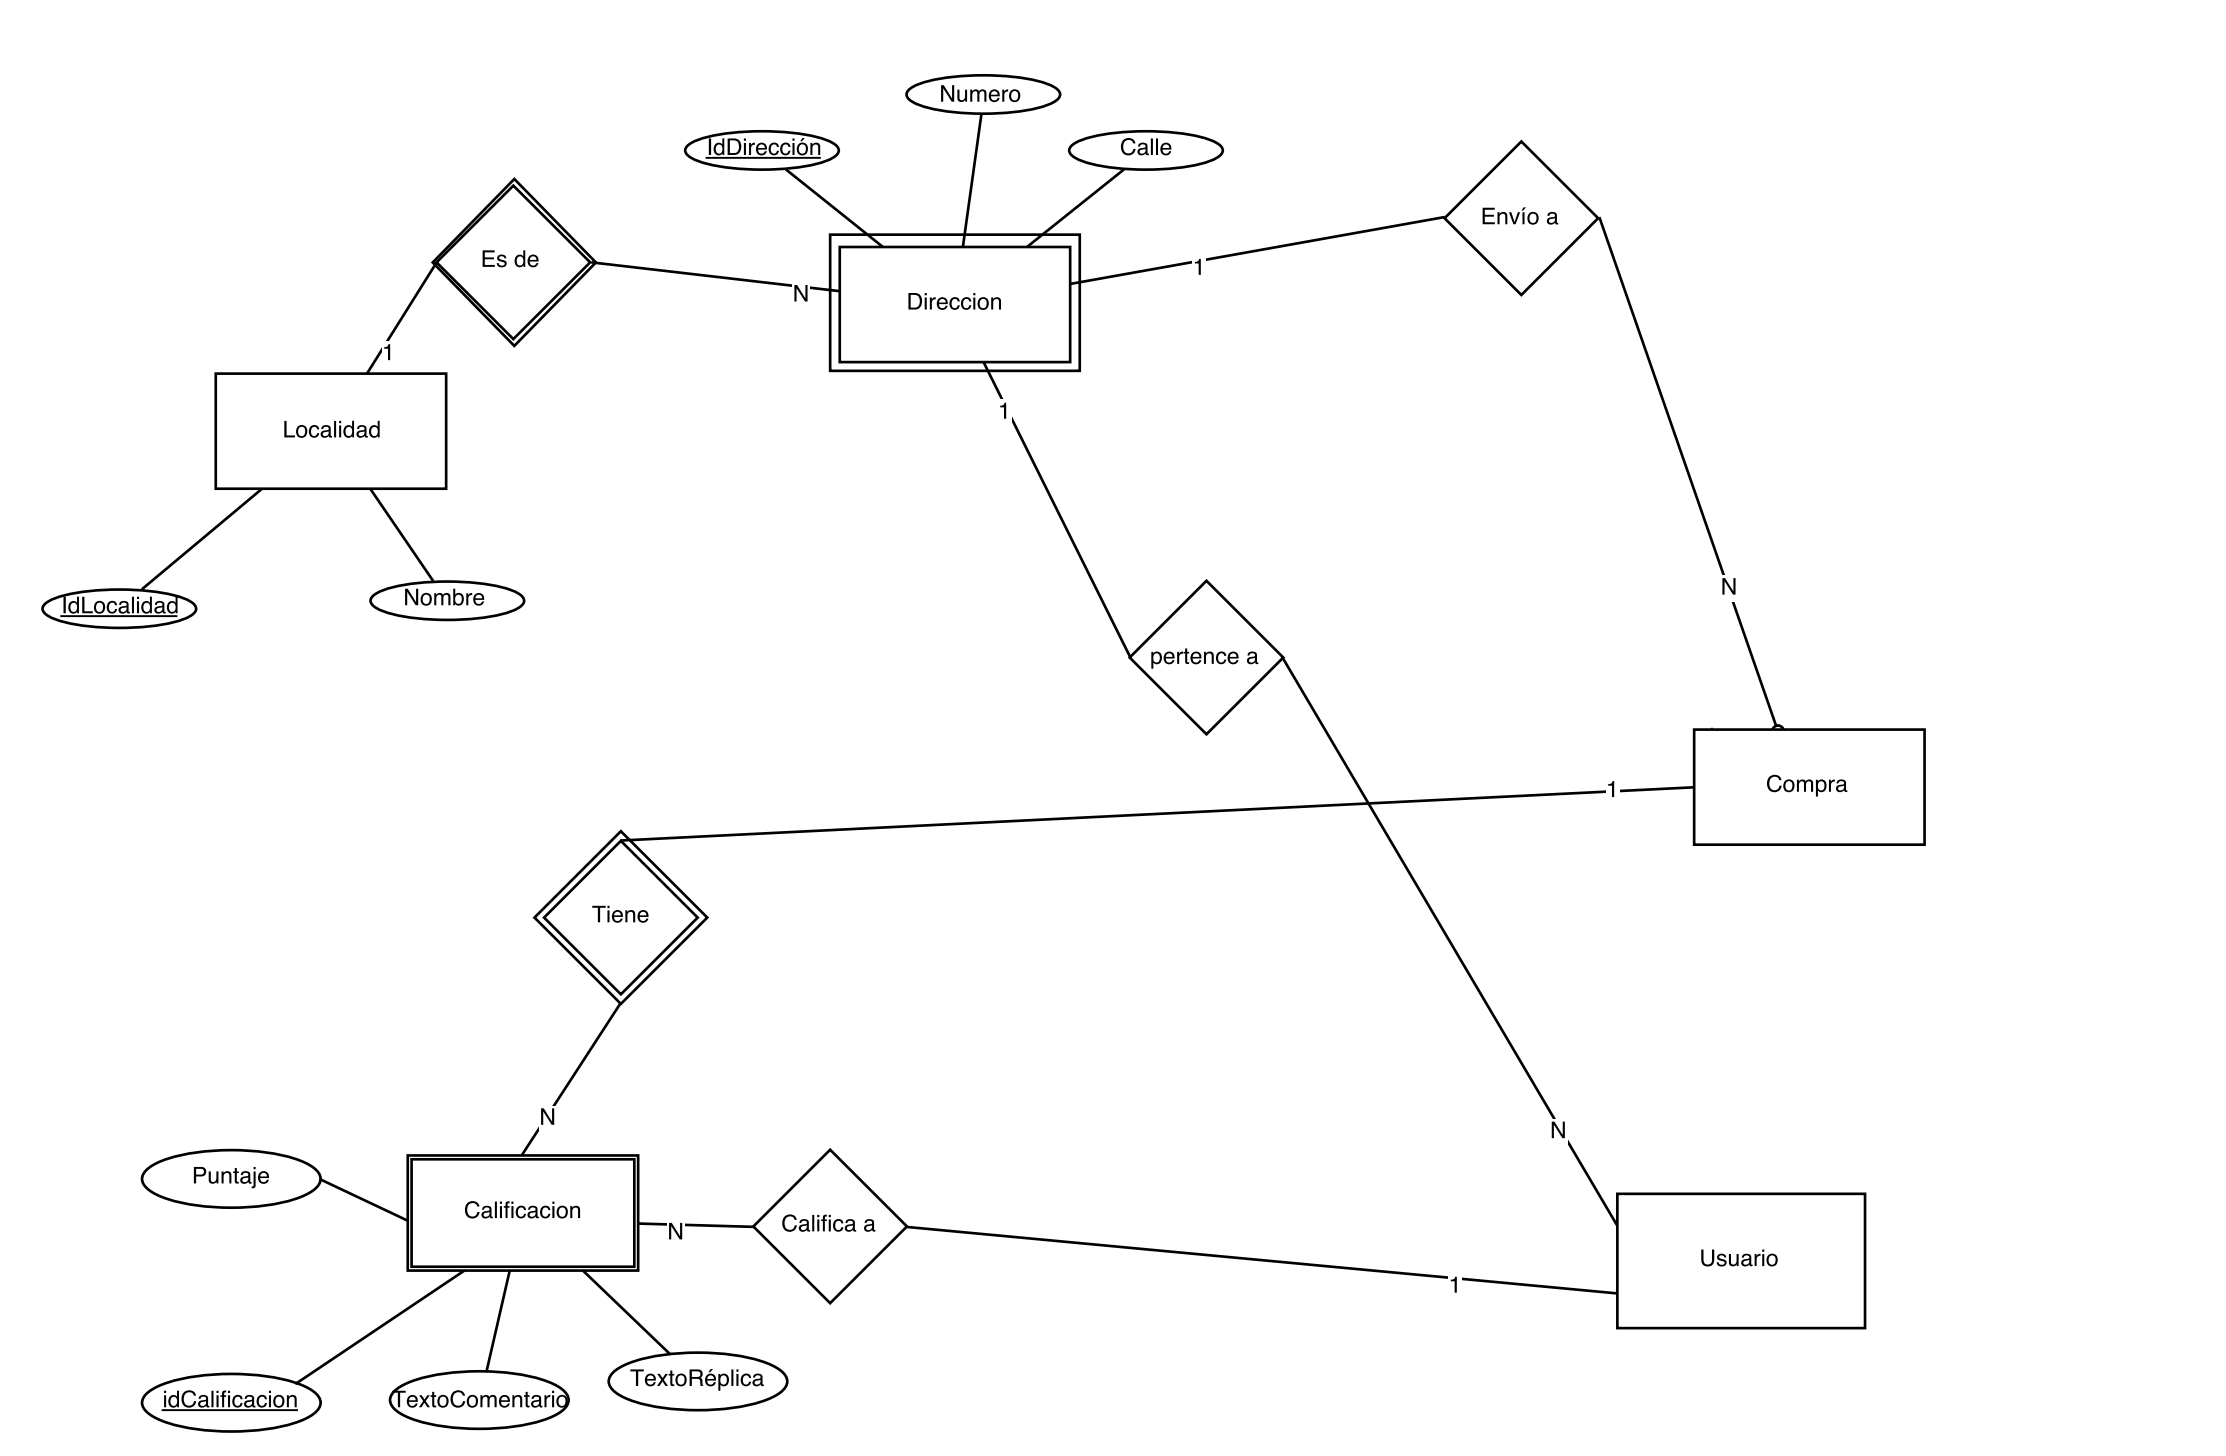
\includegraphics[width=20cm, height=12cm]{der1}
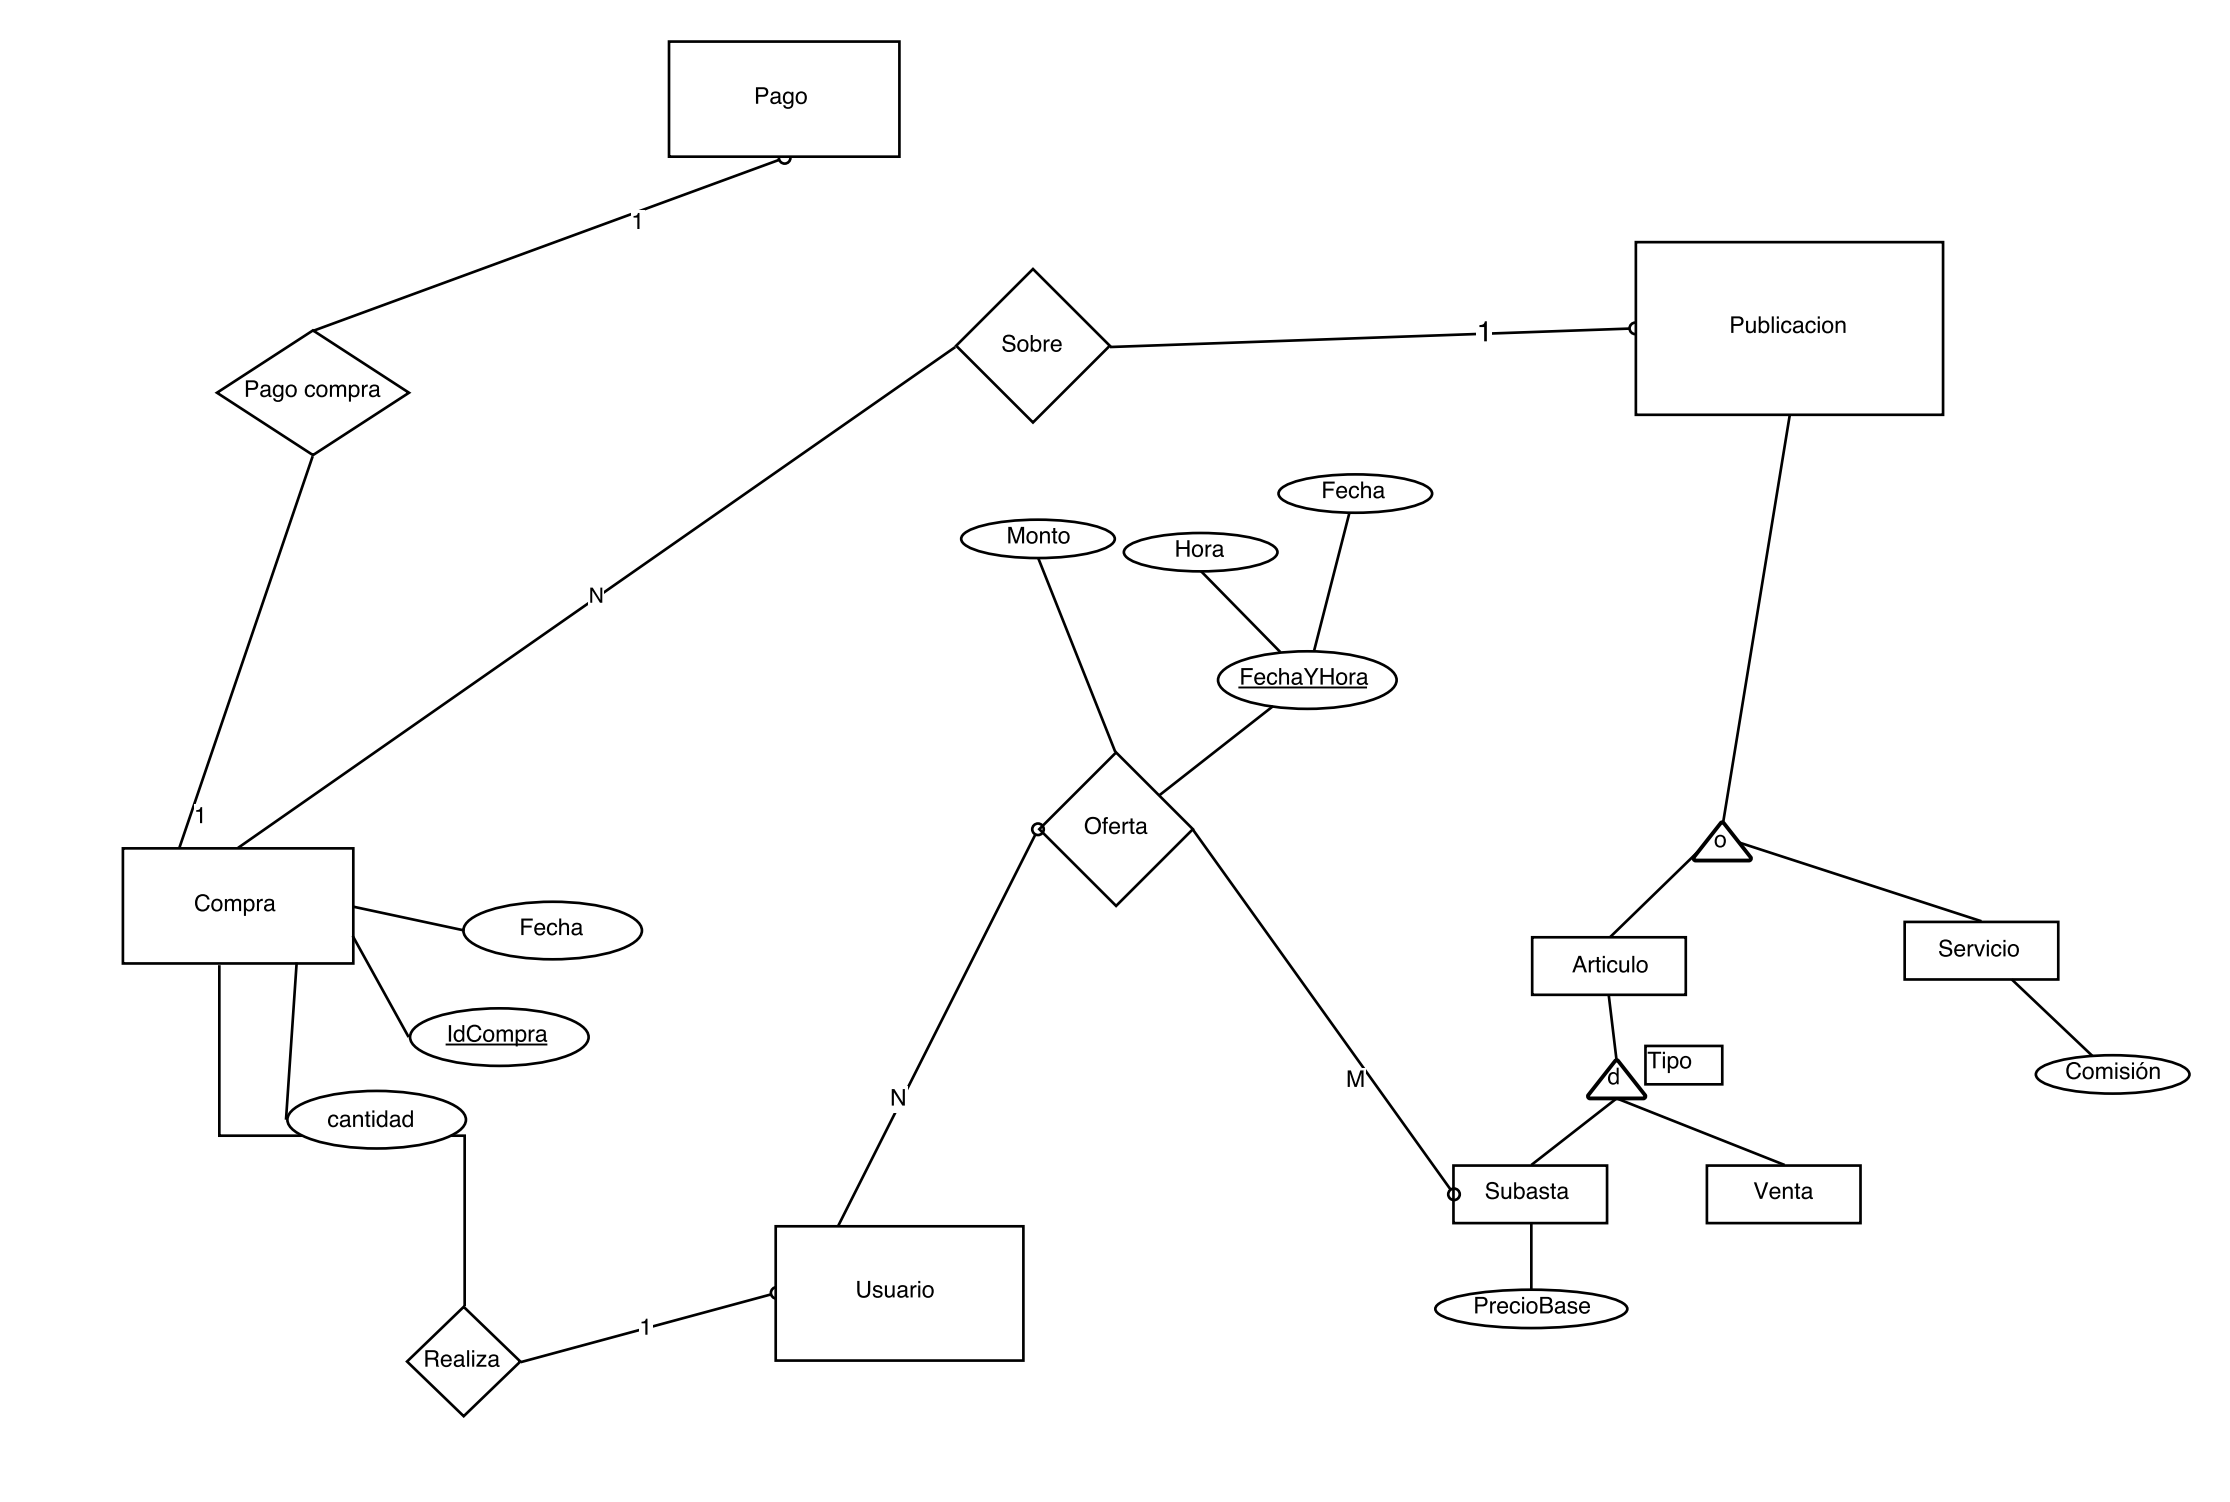
\includegraphics[width=18cm, height=12cm]{der2}
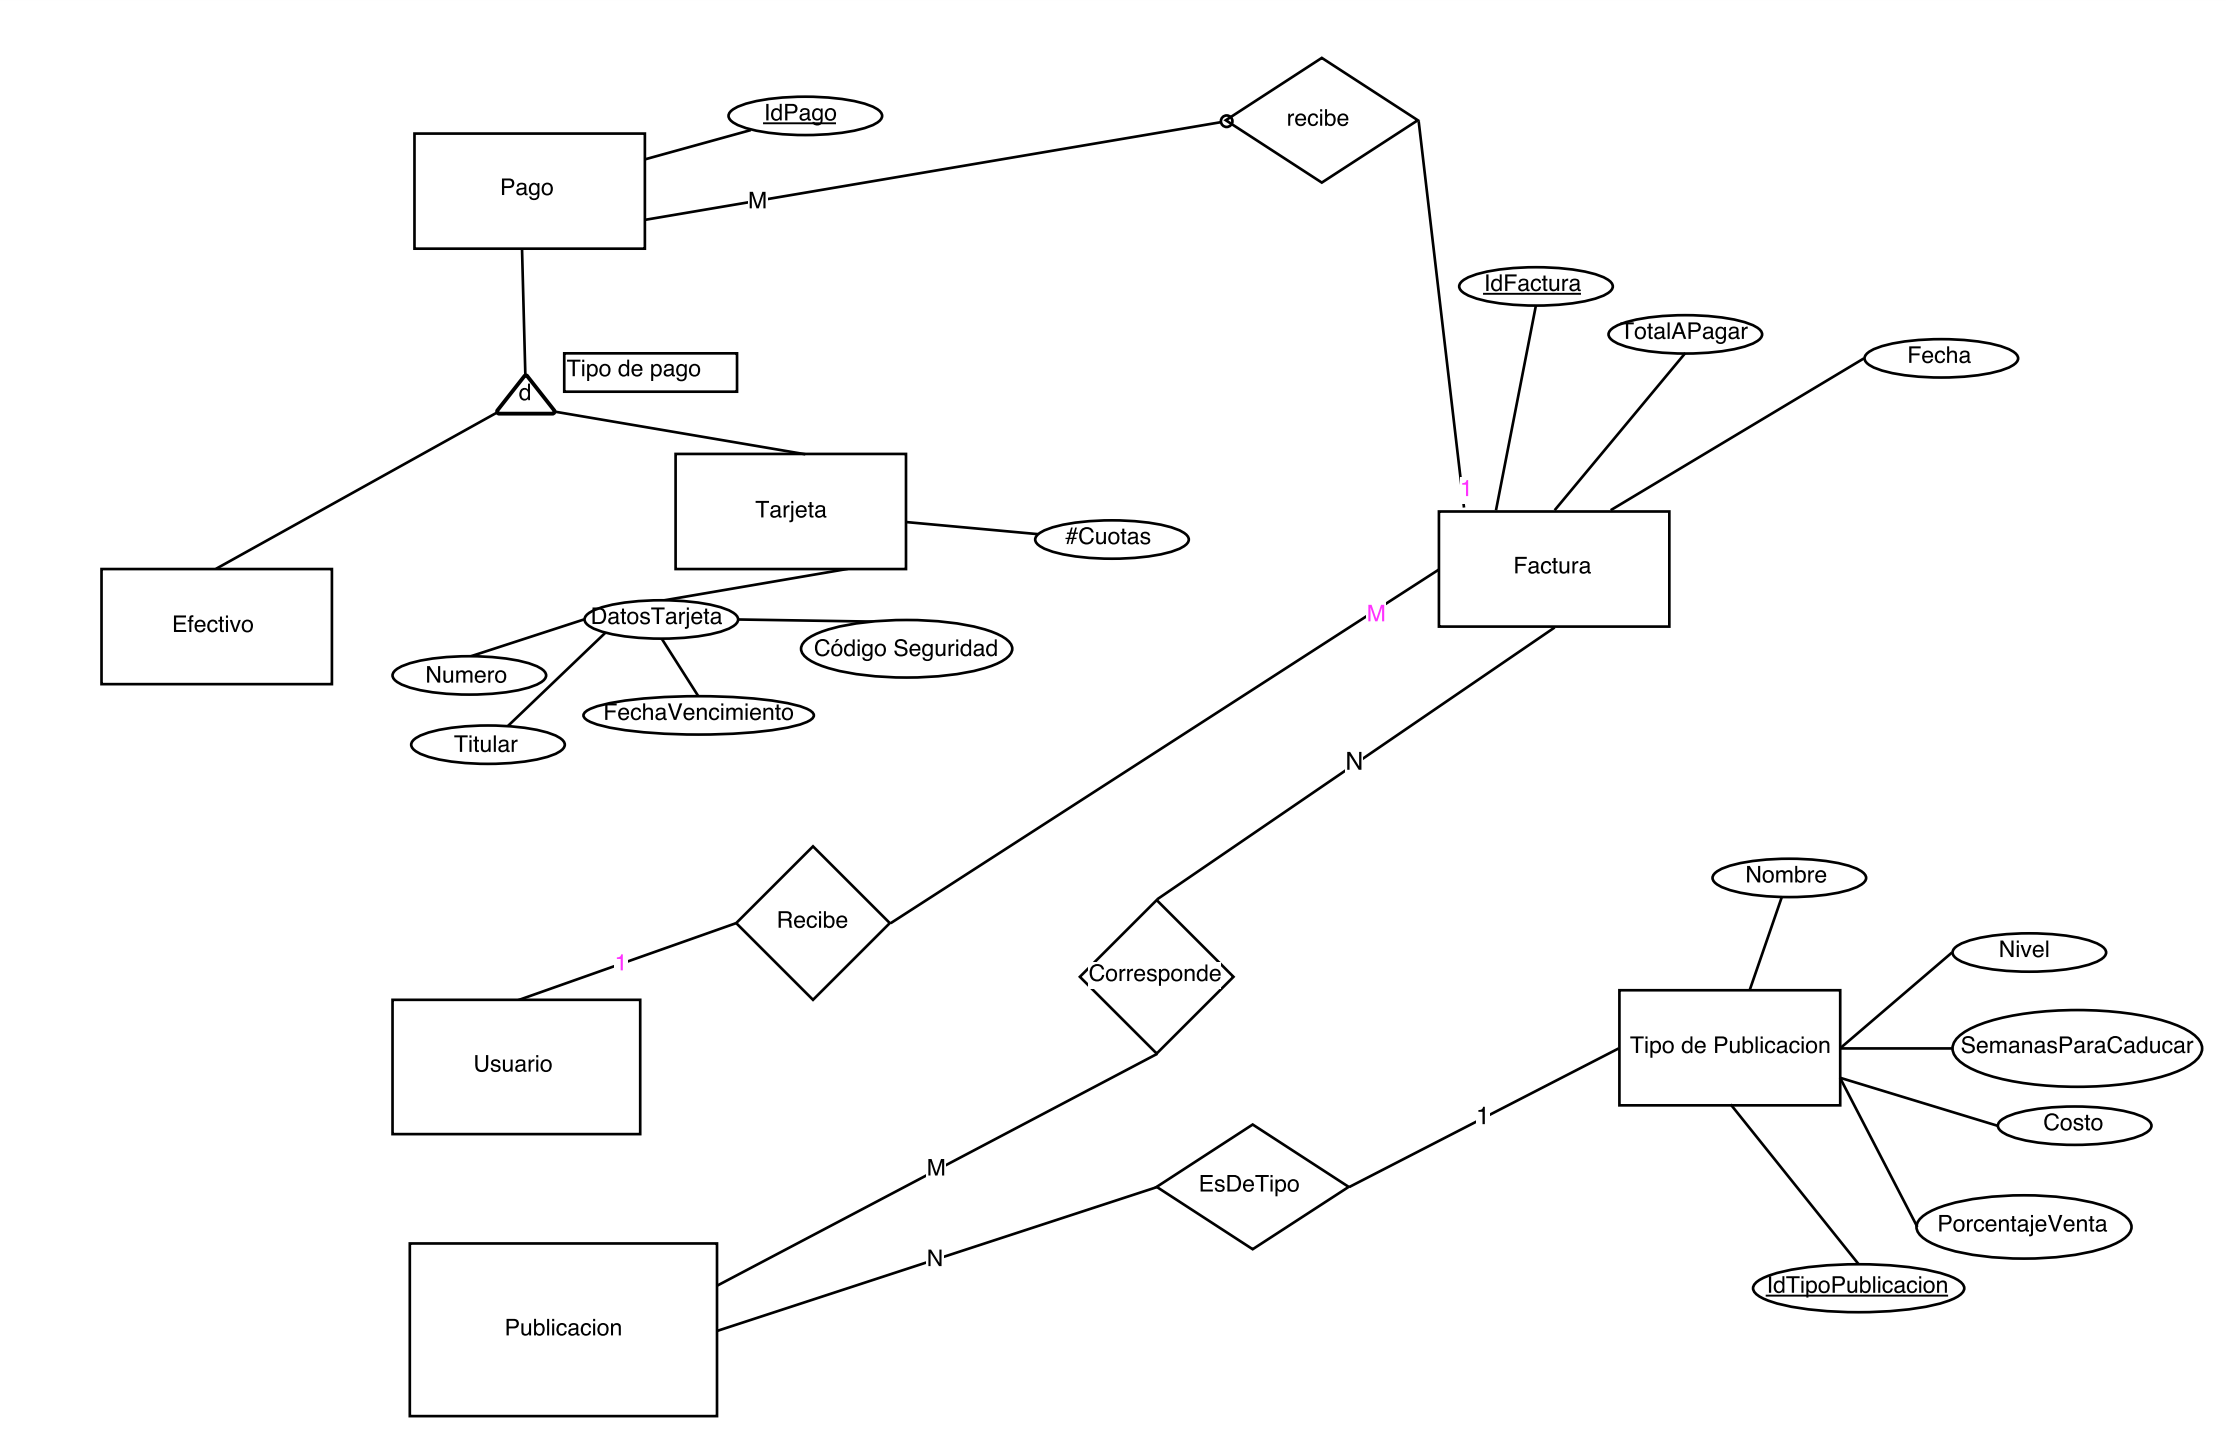
\includegraphics[width=18cm, height=12cm]{der3}
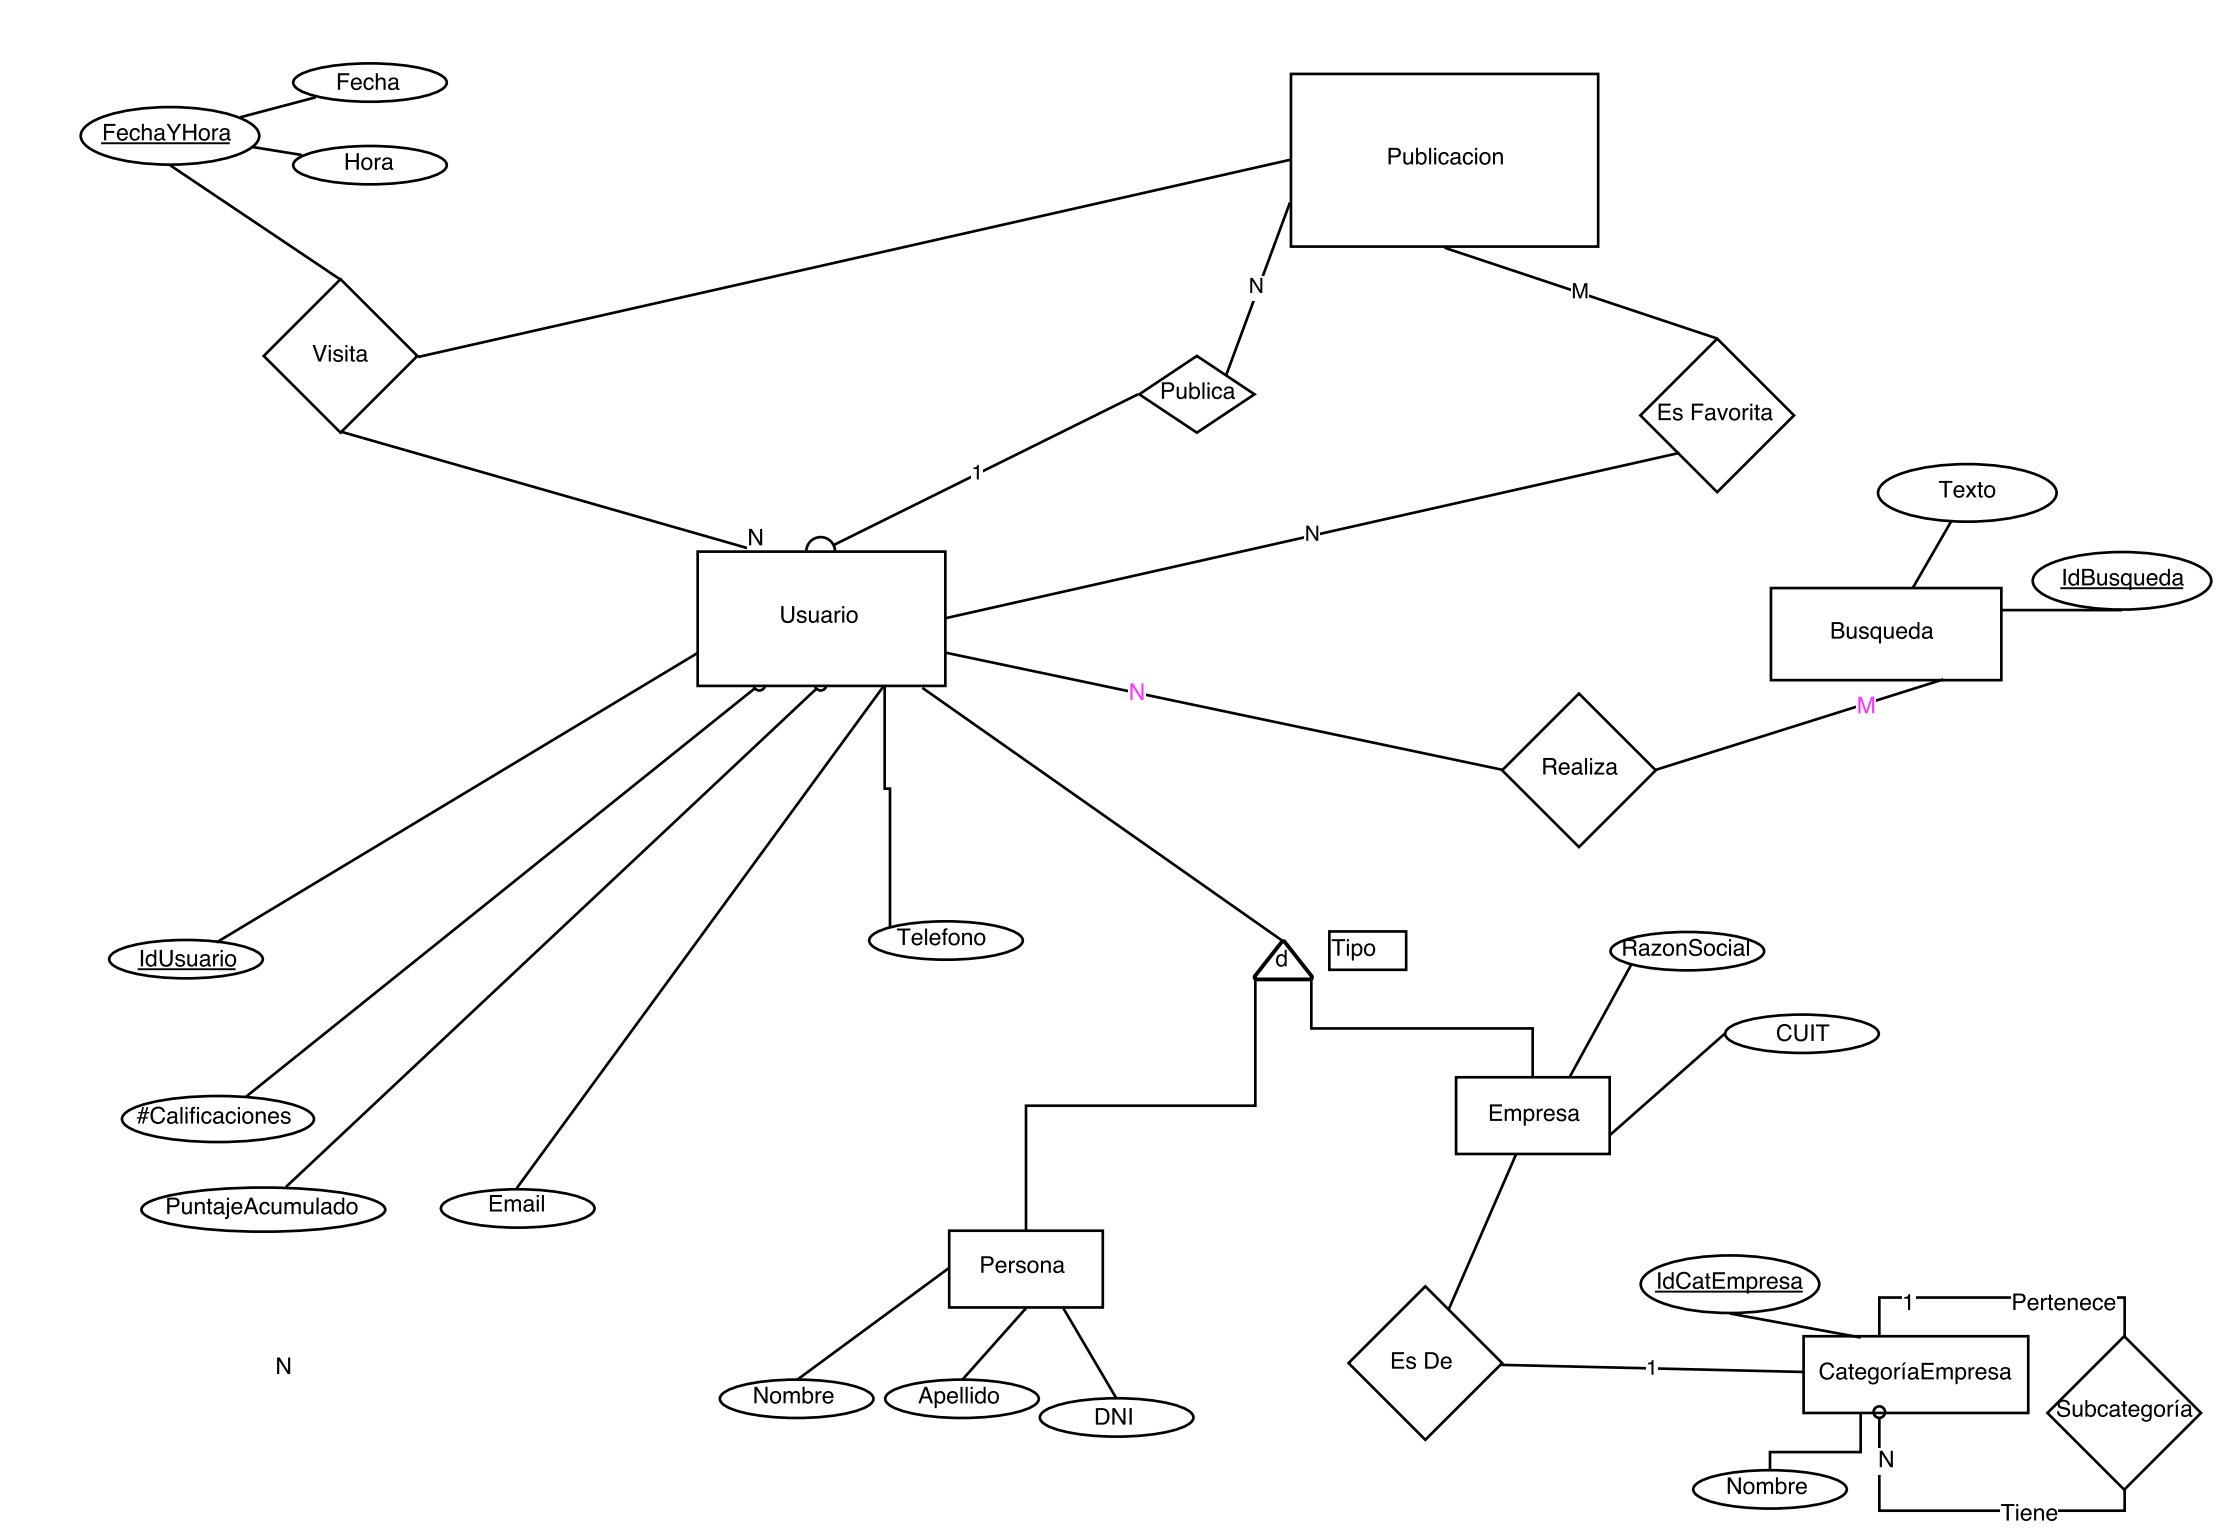
\includegraphics[width=18cm, height=12cm]{der4}
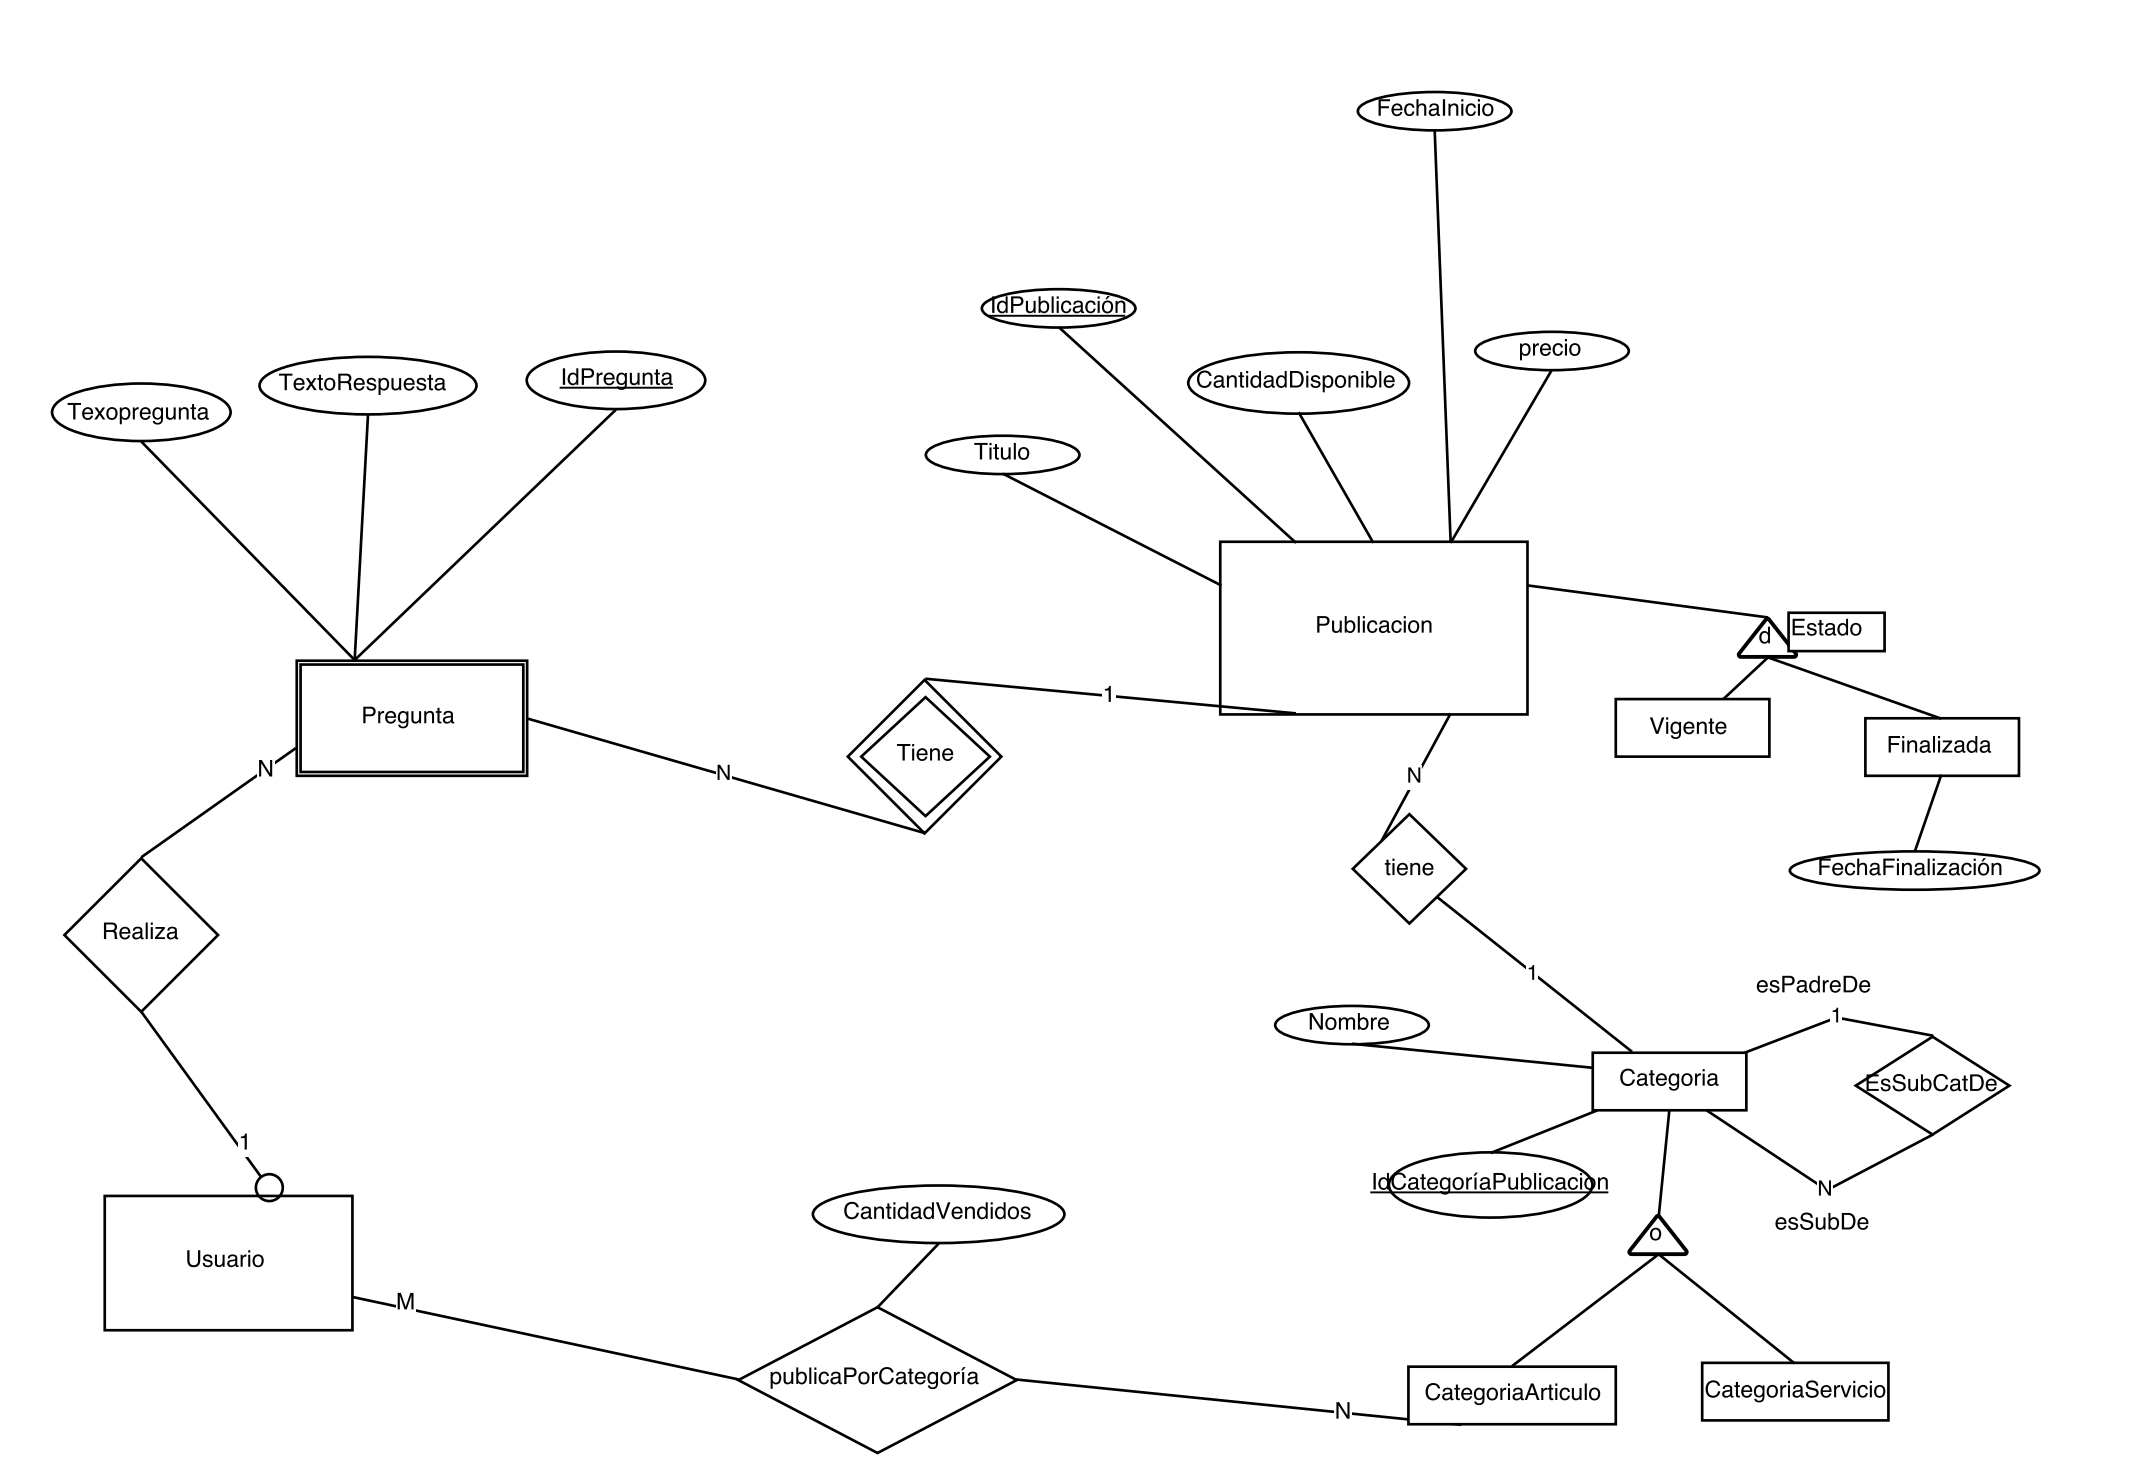
\includegraphics[width=19cm, height=12cm]{der5}

\subsection{Restricciones}

\begin{enumerate}
\item No puede haber dos DNI iguales. 
\item La publicaci\'on del tipo Libre! tiene costo 0.
\item Para cada compraventa existen a lo sumo 2 calificaciones, cada una correspondiente al comprador y vendedor.
\item El nivel de la publicaci\'on es distinto para cada tipo de publicaci\'on.
\item El usuario que compra una publicaci\'on no puede ser el usuario que publica.
\item Si un usuario realiza una respuesta a un comentario, entonces dicho comentario es de una calificaci\'on y la calificaci\'on fue hecha por un usuario que hizo dicha  compra 
\item Las publicaciones del tipo Rub\'iDelOriente aparecen primeras en las b\'usquedas. Luego aparecen en orden de mayor a menor costo de comisi\'on y por \'ultimo las de la categor\'ia Libre!.
\item El costo por mes de Rub\'iDeOriente es Fijo y se pueden hacer 3 publicaciones por mes de este tipo usuario.
\item El costo de las de Oro cobran m\'as porcentaje de la venta como comisi\'on que las de Plata
\item El costo de las de Plata cobran m\'as porcentaje de la venta como comisi\'on que las de Bronce 
\item El monto de una oferta en una subasta debe ser superior en al menos 1 peso a la oferta actual, e inferior al doble de la oferta actual
\item Una calificaci\'on tiene completado el atributo textoR\'eplica, entonces tiene completado el atributo textoComentario
\item El atributo puntaje de calificaci\'on est\'a entre [1, 10].
\item El atributo nombre de la entidad Tipo s\'olo puede ser uno de los siguientes: Rub\'iDeOriente,  Oro,  Plata,  Bronce o Libre! 
\item No se puede realizar una pregunta a una publicaci\'on que est\'a finalizada.
\item El atributo cantidad de la entidad compra siempre es menor o igual al atributo cantidadDisponible de la publicacion.
\item Si el atributo cantidadDisponible de la entidad Publicaci\'on vale 0, entonces la publicaci\'on est\'a finalizada. 
	
\item Dada una oferta, el monto de dicha oferta debe ser mayor en al menos 1 peso a todas las ofertas anteriores (en fecha), y al precioBase de la subasta. Adem\'as dicha oferta no puede superar el doble del precio base.
\item El precio de una publicaci\'on que es de tipo subasta es igual a:
el precioBase de la subasta si no hay una oferta realizada.

\item  Un usuario no puede ofertar en una publicaci\'on finalizada. 
\item  Si un usuario compr\'o una publicaci\'on de tipo subasta, entonces dicho usuario tiene que tener la oferta m\'as alta en dicha publicaci\'on. 
\item El TotalAPagar de la Factura es lo que adeuda el Usuario al sistema en concepto de abonos a Rub\'iDeOriente y/o comisi\'on por las ventas de sus programador. 
\item Un pago o se relaciona con una Publicaci\'on, o se relaciona con una Compra. Nunca con los dos.
\item El atributo CantidadVendidos de la relaci\'on publicaPorCategoria es igual a todas las ventas que realiz\'o ese usuario en esa categor\'ia.
\item El tipo dentro de la tabla Articulo puede ser o venta o subaste 

\end{enumerate}


%%%%%%%%%%%%%%%%%%%%%%%%%%%%%%%%%%%%%%%%%%%%%%%%%%%%%%%%%%%%%%%%%%%%%%%%%%%%%%%
%% Modelo Relacional                                                         %%
%%%%%%%%%%%%%%%%%%%%%%%%%%%%%%%%%%%%%%%%%%%%%%%%%%%%%%%%%%%%%%%%%%%%%%%%%%%%%%%


\section{Modelo Relacional}


\relacion{Facultad}{
  \pk{idFacultad},
  nombre
}{
  \clavespkck{idFacultad}
}

\relacion{Empadronado}{
  \pk{DNI},
  nombre,
  fechaDeNacimiento,
  \fk{idFacultad},
  claustro
}{
  \clavespkck{DNI}
}

\relacion{Estudiante}{
  \pkfk{DNI},
  fechaDeInscripcion
}{
  \clavespkckfk{DNI}
}

\relacion{Graduado}{
  \pkfk{DNI},
  universidad
}{
  \clavespkckfk{DNI}
}

\section{Suposiciones}

\section{Diseno Fisico}

\section{Codigo}

\section{Conclusiones}


\end{document}
